\documentclass{article}
\usepackage[T1]{fontenc}
\usepackage[utf8]{inputenc}
\usepackage[polish]{babel}
\usepackage{amsmath}
\usepackage{amssymb}
\usepackage{graphicx}
\usepackage{booktabs}
\usepackage{float}
\usepackage{array}
\graphicspath{{plots/}}

\author{
    Mateusz Kosowski 251558 \\
    Nikodem Nowak 251598 \\
dr inż. Marcin Kacprowicz
}
\title{Załączniki do sprawozdania\\Projekt 2. Podsumowania lingwistyczne relacyjnych baz danych}

\begin{document}
\maketitle

\noindent Niniejszy dokument zawiera załączniki do sprawozdania głównego:
zestawienie miar jakości ($T_1$--$T_{11}$), pomocnicze diagramy UML oraz
wykresy funkcji przynależności zmiennych lingwistycznych i~kwantyfikatorów.
Zgodnie z~regulaminem załączniki nie wliczają się do limitu 20 stron
sprawozdania.

\appendix
\section{Miary jakości podsumowań -- zestawienie}
\label{app:measures}

\begin{table}[H]
\centering
\caption{Jedenaście miar jakości podsumowania lingwistycznego użytych
w~eksperymentach (\S4 sprawozdania głównego) wraz z~ich skrótowym znaczeniem
(definicje: Yager 1982; Kacprzyk, Yager 2001; Zadrożny 2006; Niewiadomski 2008).
Miary $T_9$--$T_{11}$ dotyczą wyłącznie kwalifikatora, więc dla formy~I
(bez kwalifikatora) są tożsamościowo równe~$0$.}
\label{tab:measures}
\begin{tabular}{l p{0.78\textwidth}}
\toprule
Miara & Znaczenie (czego dotyczy, kiedy wysoka) \\
\midrule
$T_1$ & stopień prawdziwości -- jak bardzo zdanie jest prawdziwe na danych \\
$T_2$ & nieprecyzyjność sumaryzatora -- wysoka, gdy etykiety mają wąskie nośniki \\
$T_3$ & stopień pokrycia -- udział rekordów realnie wpadających w~sumaryzator \\
$T_4$ & stopień trafności -- rozbieżność pokryć atomów (istotna dla sumaryzatorów złożonych) \\
$T_5$ & długość (zwięzłość) sumaryzatora -- maleje z~liczbą połączonych etykiet \\
$T_6$ & nieprecyzyjność kwantyfikatora -- wysoka dla kwantyfikatora o~wąskim nośniku \\
$T_7$ & kardynalność kwantyfikatora -- jw., liczona przez $\sigma$-count \\
$T_8$ & kardynalność sumaryzatora -- ,,ostrość'' etykiet sumaryzatora ($\sigma$-count) \\
$T_9$ & nieprecyzyjność kwalifikatora -- jak $T_2$, lecz dla kwalifikatora \\
$T_{10}$ & kardynalność kwalifikatora -- jak $T_8$, lecz dla kwalifikatora \\
$T_{11}$ & długość (zwięzłość) kwalifikatora \\
\bottomrule
\end{tabular}
\end{table}

\section{Pomocnicze diagramy UML}
\label{app:uml}

Poniższe diagramy uzupełniają opis architektury z~\S3 sprawozdania głównego.
Do raportu głównego przeniesiono tylko diagramy bezpośrednio związane
z generowaniem podsumowań, natomiast tutaj pozostawiono warstwę rozmytą,
dostęp do danych oraz interfejs graficzny.

\begin{figure}[H]
\centering
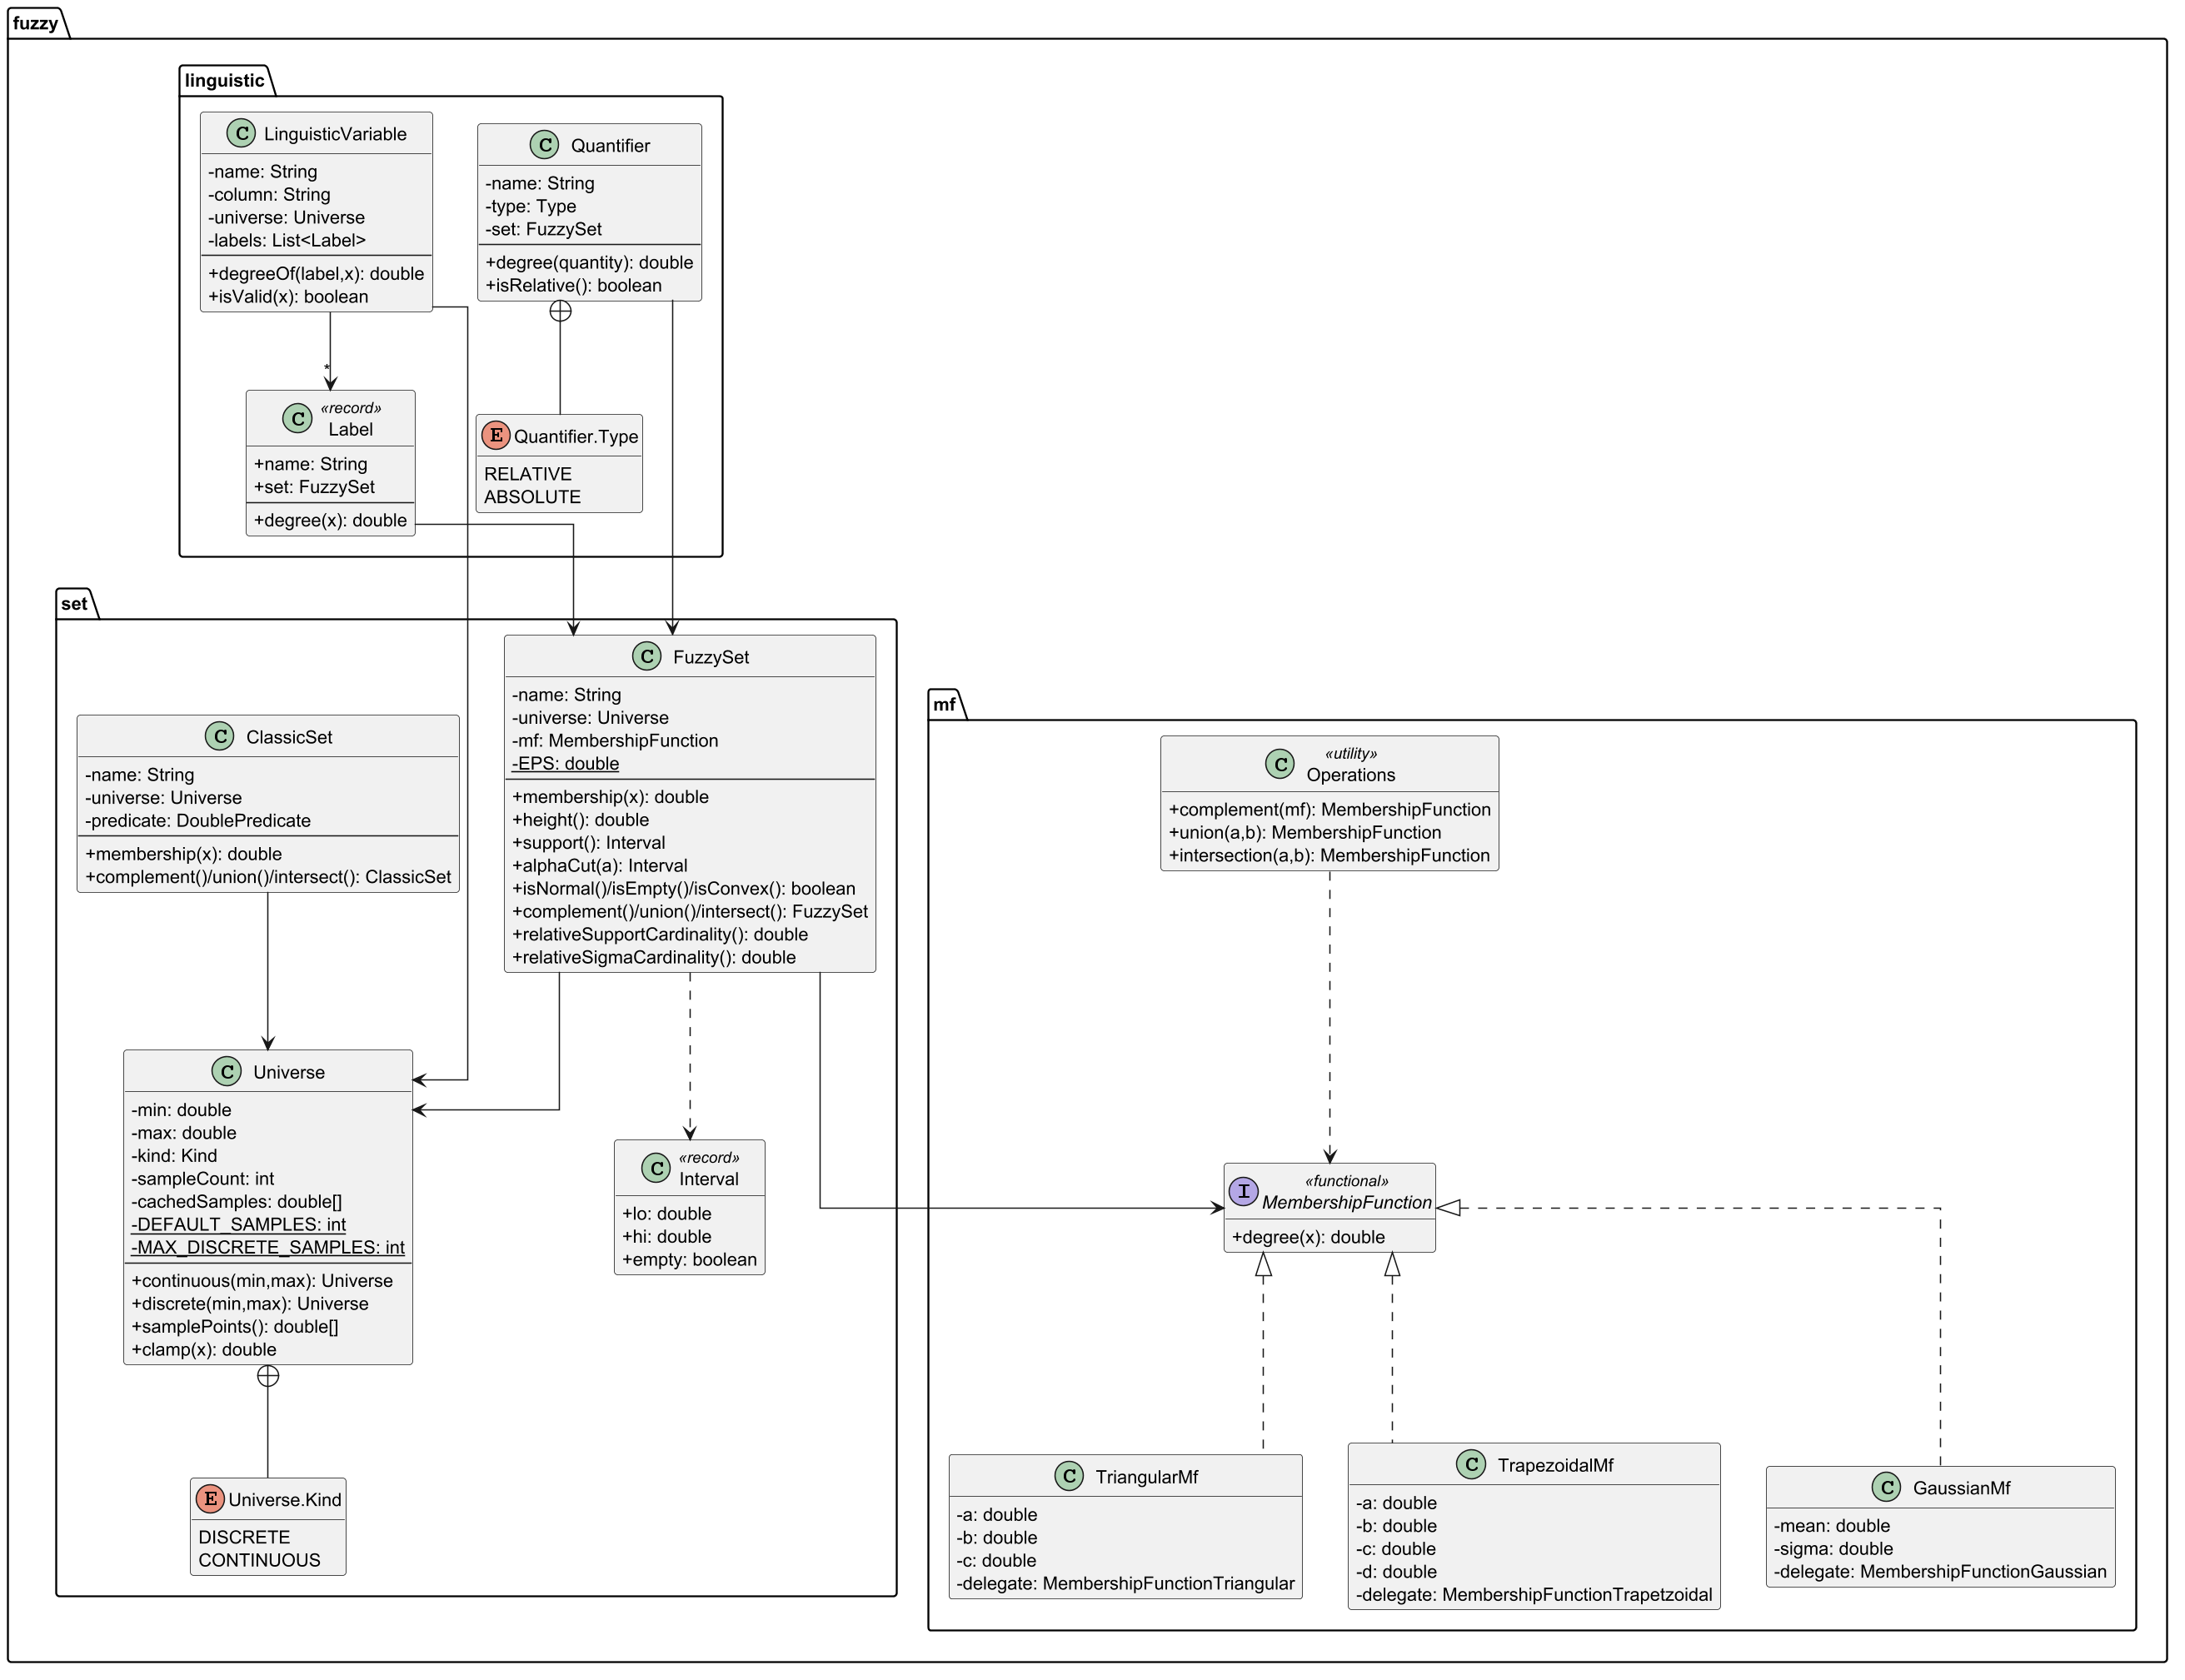
\includegraphics[width=0.9\textwidth]{uml_fuzzy.png}
\caption{Diagram klas pakietów rozmytych: \texttt{fuzzy.set},
\texttt{fuzzy.mf} i~\texttt{fuzzy.linguistic}.}
\label{fig:app-uml-fuzzy}
\end{figure}

\begin{figure}[H]
\centering
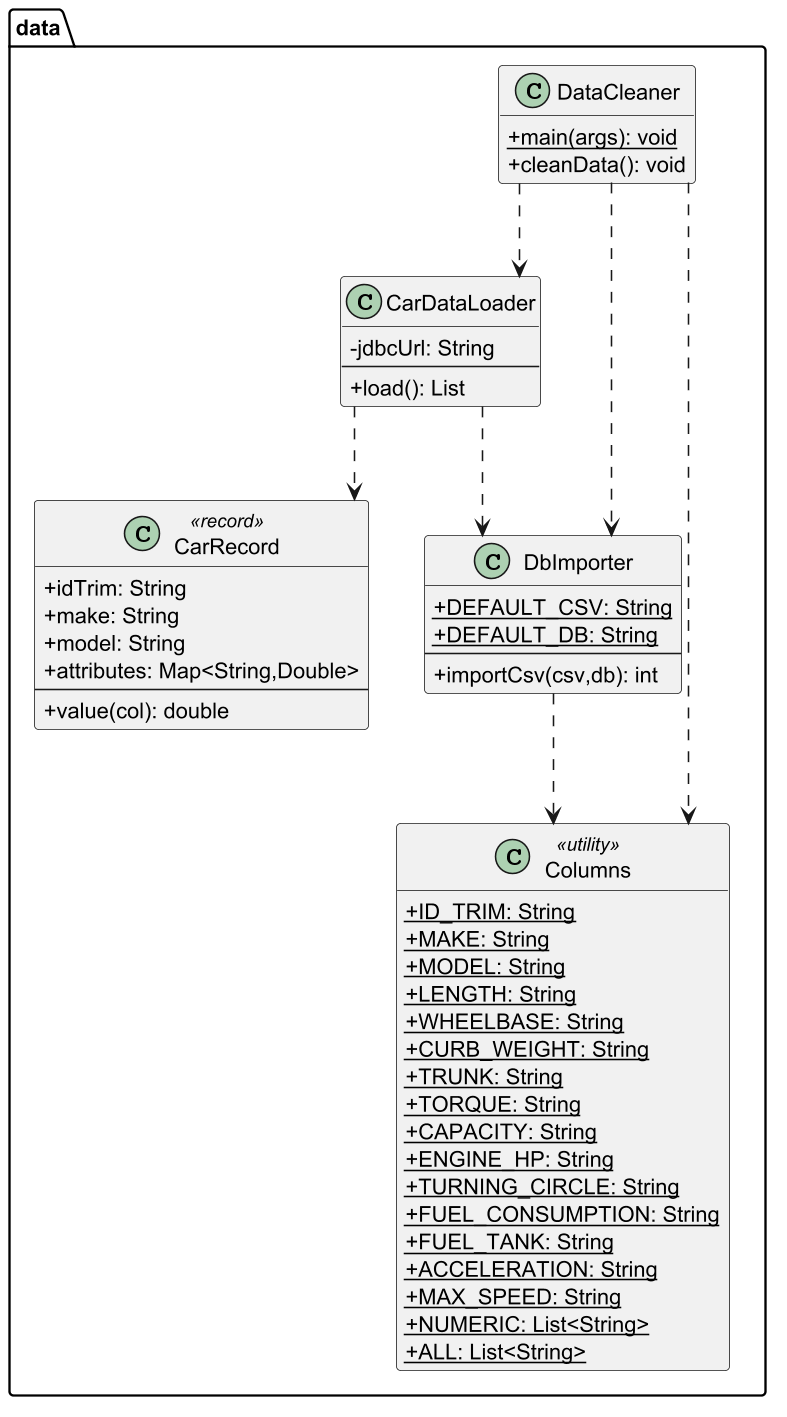
\includegraphics[width=0.9\textwidth]{uml_data.png}
\caption{Diagram klas warstwy danych: import, czyszczenie i odczyt rekordów
samochodów z bazy SQLite.}
\label{fig:app-uml-data}
\end{figure}

\begin{figure}[H]
\centering
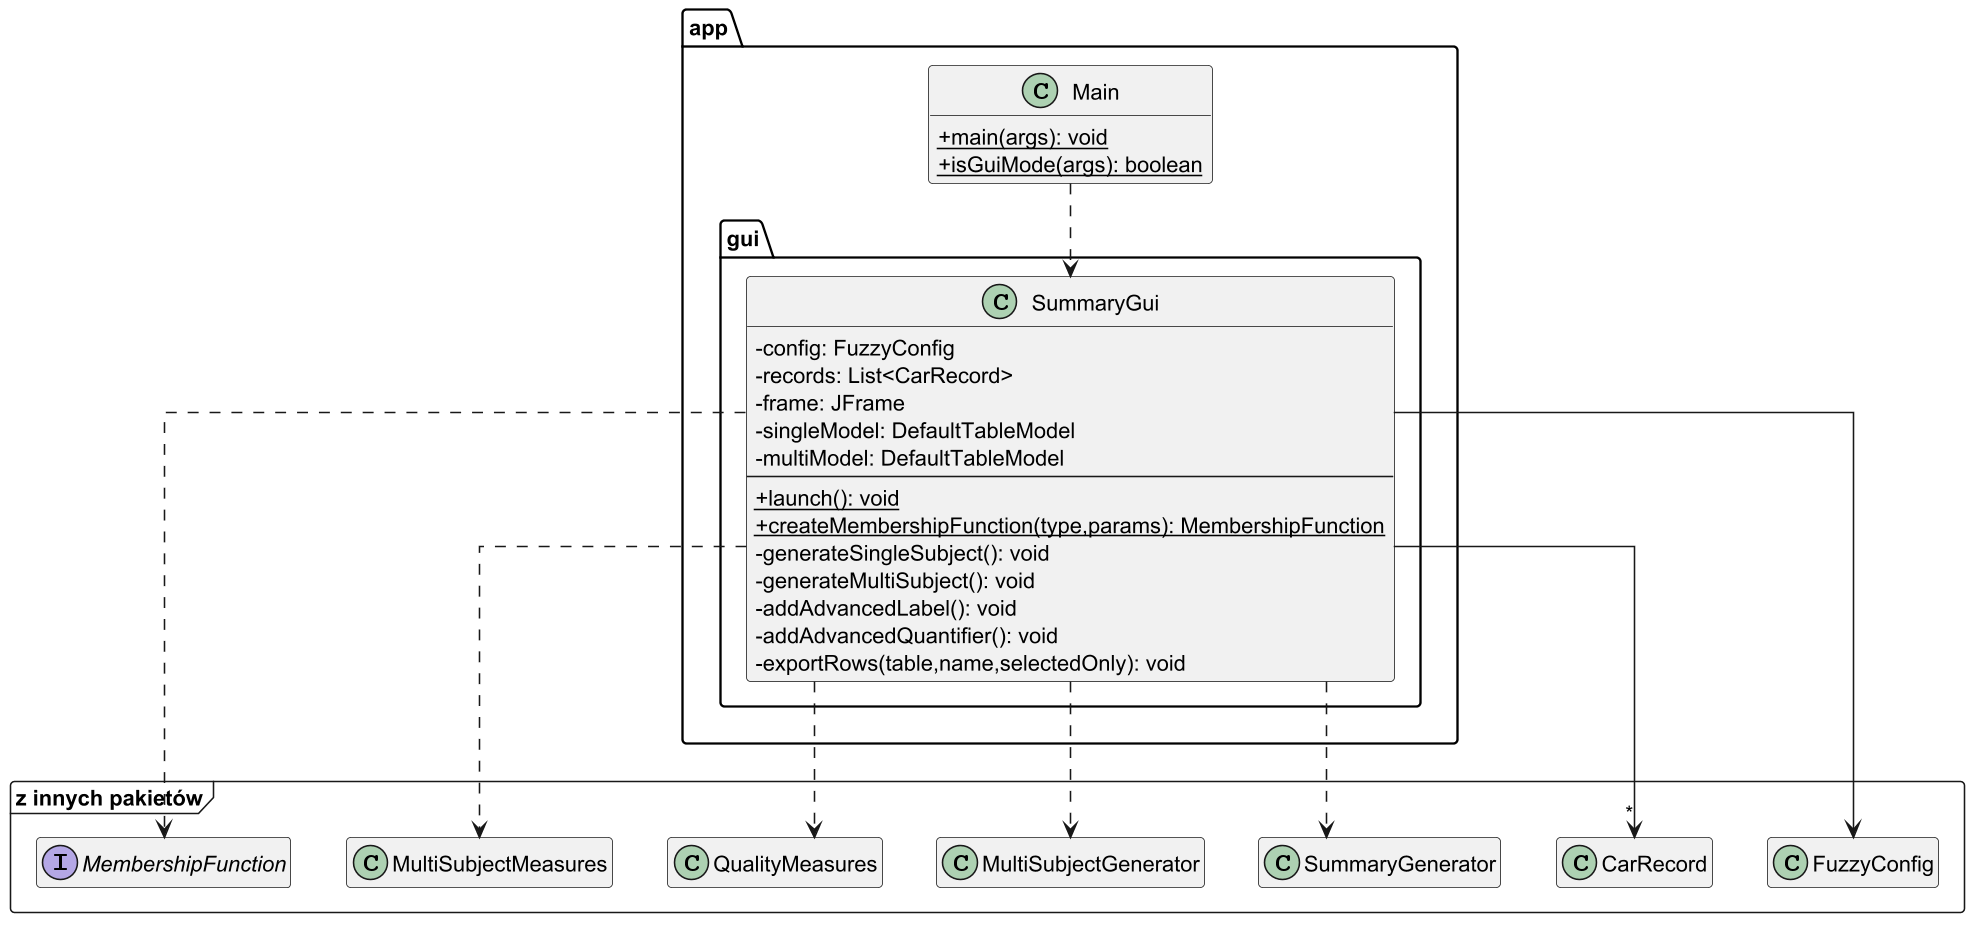
\includegraphics[width=0.9\textwidth]{uml_gui.png}
\caption{Diagram klasy interfejsu graficznego aplikacji.}
\label{fig:app-uml-gui}
\end{figure}

\section{Wykresy funkcji przynależności zmiennych lingwistycznych i~kwantyfikatorów}
\label{app:plots}

Załącznik zbiera wykresy funkcji przynależności wszystkich $12$ zmiennych
lingwistycznych oraz obu rodzin kwantyfikatorów (zdefiniowanych w~\S2
sprawozdania głównego). Linią ciągłą zaznaczono funkcję przynależności każdej
etykiety, a~wypełnieniem -- jej obszar wsparcia. Parametry $(a,b,c,d)$
wszystkich trapezów podano w~tabelach parametrów w~\S2 sprawozdania głównego.
Zgodnie z~regulaminem załączniki nie wliczają się do limitu stron sprawozdania.

\begin{figure}[H]
\centering
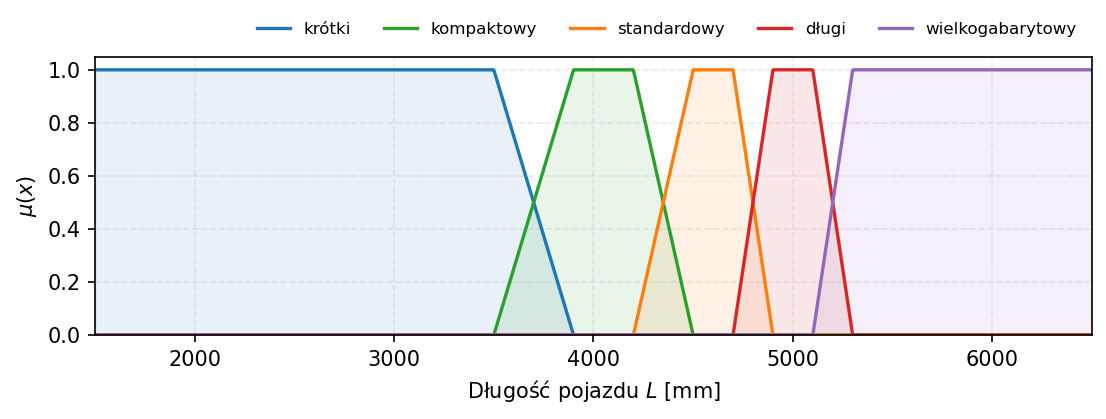
\includegraphics[width=0.9\textwidth]{mf_length_mm.png}
\caption{Funkcje przynależności pięciu etykiet zmiennej lingwistycznej
,,długość pojazdu'' $L \in [1500,6500]$~mm. Granice etykiet odpowiadają
segmentom Euro: A ($<$3,7 m), B (3,7--4,5 m), C/D (4,5--4,9 m),
E (4,9--5,3 m), F ($>$5,3 m).}
\label{fig:mf-length}
\end{figure}

\begin{figure}[H]
\centering
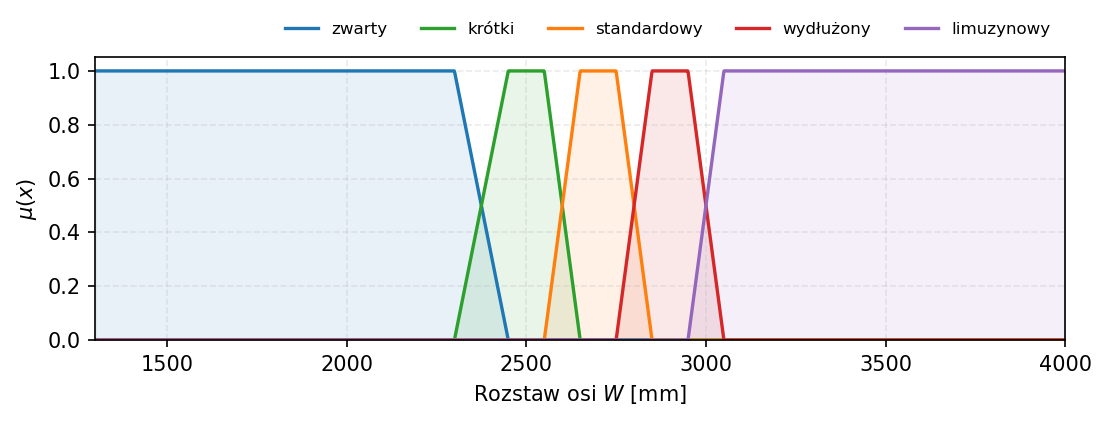
\includegraphics[width=0.9\textwidth]{mf_wheelbase_mm.png}
\caption{Funkcje przynależności pięciu etykiet zmiennej lingwistycznej
,,rozstaw osi'' $W \in [1300, 4000]$~mm.}
\label{fig:mf-wheelbase}
\end{figure}

\begin{figure}[H]
\centering
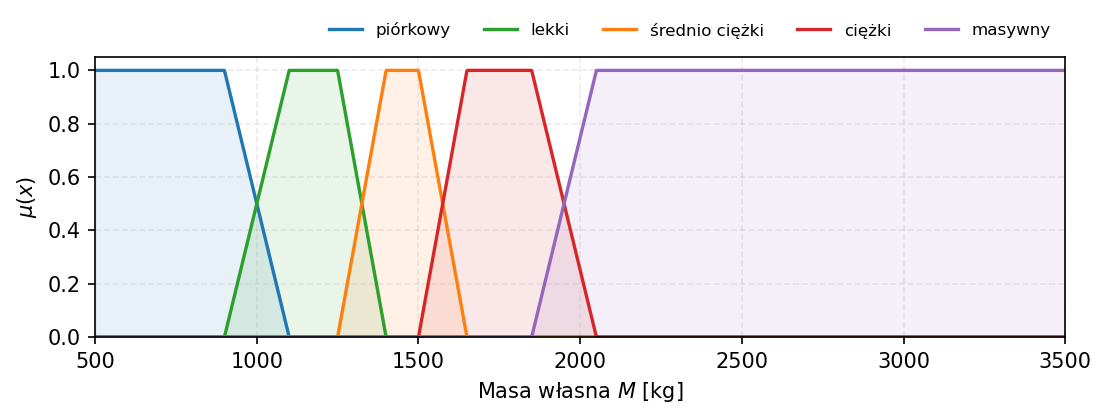
\includegraphics[width=0.9\textwidth]{mf_curb_weight_kg.png}
\caption{Funkcje przynależności pięciu etykiet zmiennej lingwistycznej
,,masa własna pojazdu'' $M \in [500, 3500]$~kg.}
\label{fig:mf-mass}
\end{figure}

\begin{figure}[H]
\centering
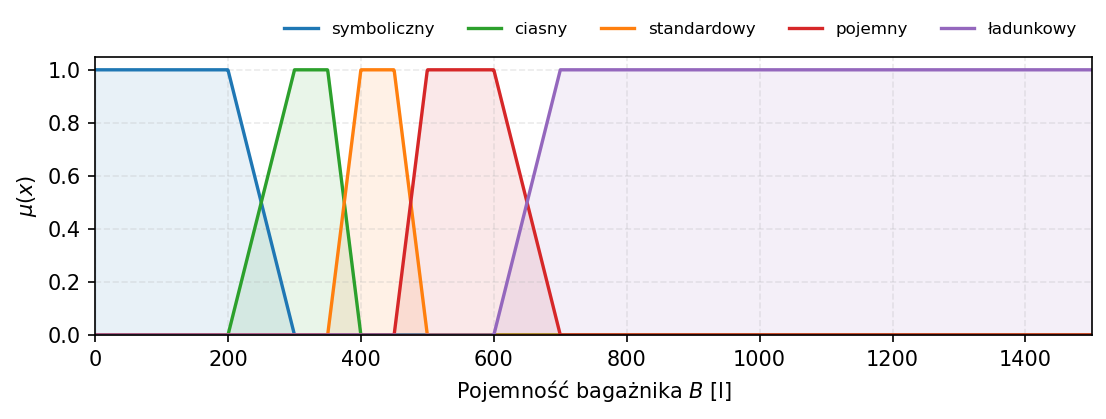
\includegraphics[width=0.9\textwidth]{mf_minimum_trunk_capacity_l.png}
\caption{Funkcje przynależności pięciu etykiet zmiennej lingwistycznej
,,pojemność bagażnika'' $B \in [0, 1500]$~l.}
\label{fig:mf-trunk}
\end{figure}

\begin{figure}[H]
\centering
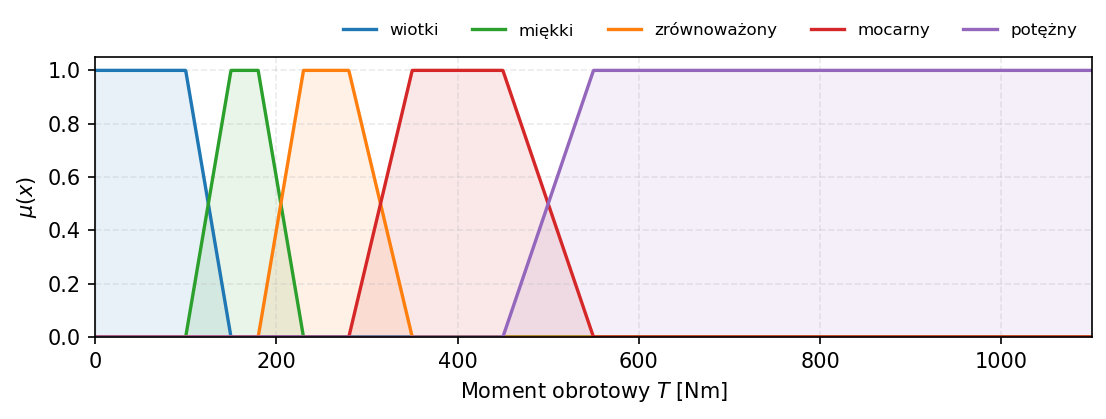
\includegraphics[width=0.9\textwidth]{mf_maximum_torque_n_m.png}
\caption{Funkcje przynależności pięciu etykiet zmiennej lingwistycznej
,,maksymalny moment obrotowy'' $T \in [0, 1100]$~Nm.}
\label{fig:mf-torque}
\end{figure}

\begin{figure}[H]
\centering
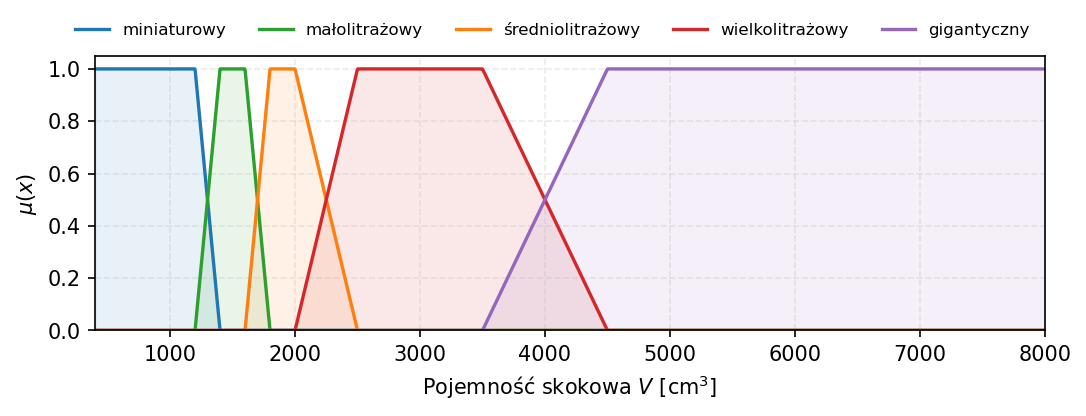
\includegraphics[width=0.9\textwidth]{mf_capacity_cm3.png}
\caption{Funkcje przynależności pięciu etykiet zmiennej lingwistycznej
,,pojemność skokowa silnika'' $V \in [400, 8000]$~cm$^3$.}
\label{fig:mf-capacity}
\end{figure}

\begin{figure}[H]
\centering
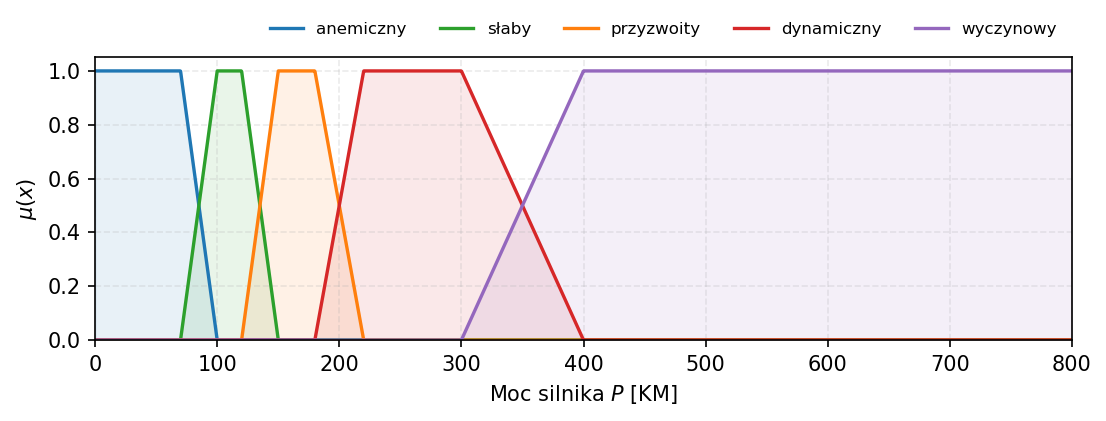
\includegraphics[width=0.9\textwidth]{mf_engine_hp.png}
\caption{Funkcje przynależności pięciu etykiet zmiennej lingwistycznej
,,moc silnika'' $P \in [0, 800]$~KM. Zauważalne liniowe przejścia
w~punktach 50\,\%-stopnia przynależności (np. dla $P=100$~KM:
$\mu_{\text{anemiczny}}(P)=\mu_{\text{słaby}}(P)=0{,}5$) ilustrują rozmyte
pokrycie zupełne wymagane konstrukcją trapezów.}
\label{fig:mf-engine-hp}
\end{figure}

\begin{figure}[H]
\centering
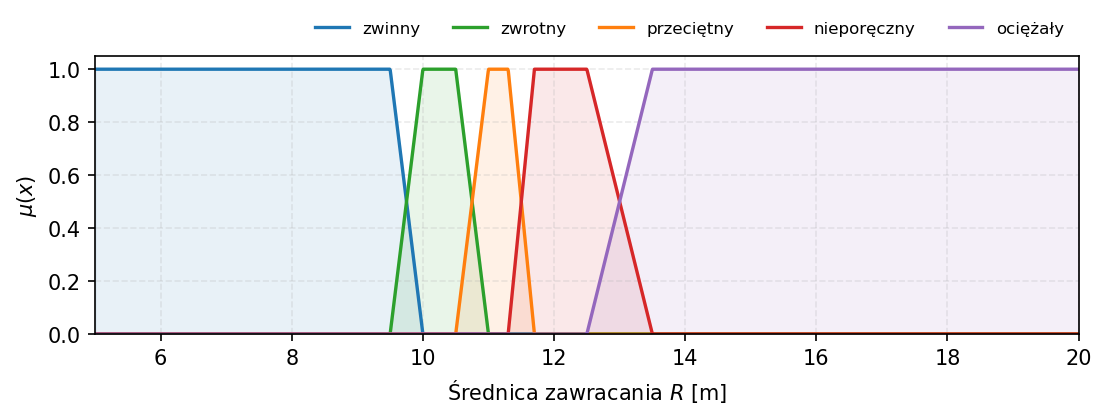
\includegraphics[width=0.9\textwidth]{mf_turning_circle_m.png}
\caption{Funkcje przynależności pięciu etykiet zmiennej lingwistycznej
,,średnica zawracania'' $R \in [5, 20]$~m.}
\label{fig:mf-turn}
\end{figure}

\begin{figure}[H]
\centering
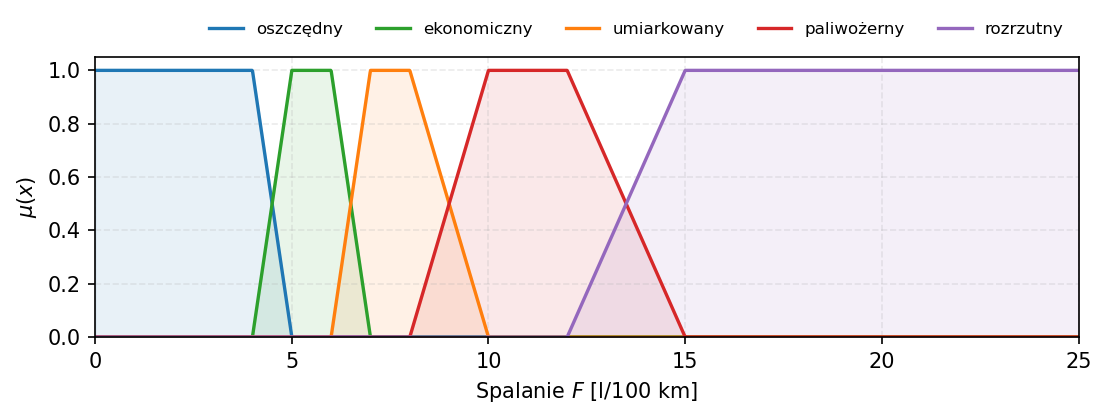
\includegraphics[width=0.9\textwidth]{mf_mixed_fuel_consumption_per_100_km_l.png}
\caption{Funkcje przynależności pięciu etykiet zmiennej lingwistycznej
,,spalanie mieszane'' $F \in [0, 25]$~l/100~km.}
\label{fig:mf-fuel}
\end{figure}

\begin{figure}[H]
\centering
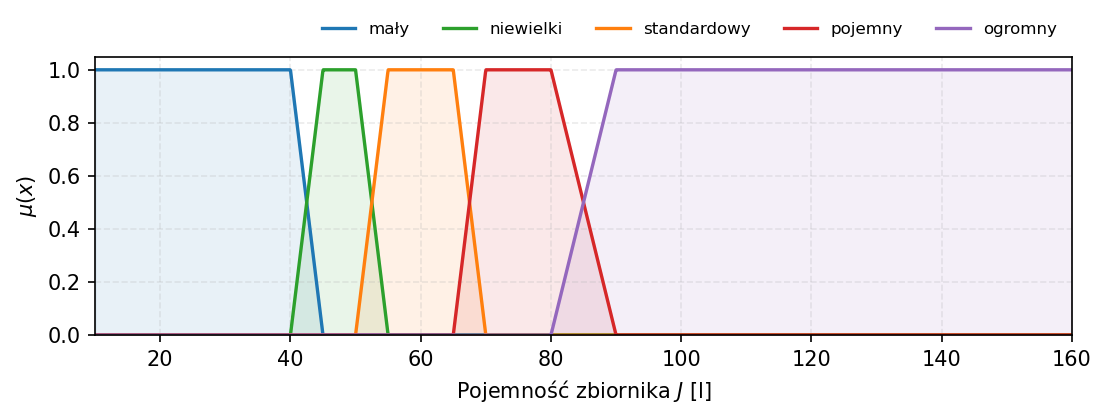
\includegraphics[width=0.9\textwidth]{mf_fuel_tank_capacity_l.png}
\caption{Funkcje przynależności pięciu etykiet zmiennej lingwistycznej
,,pojemność zbiornika paliwa'' $J \in [10, 160]$~l.}
\label{fig:mf-tank}
\end{figure}

\begin{figure}[H]
\centering
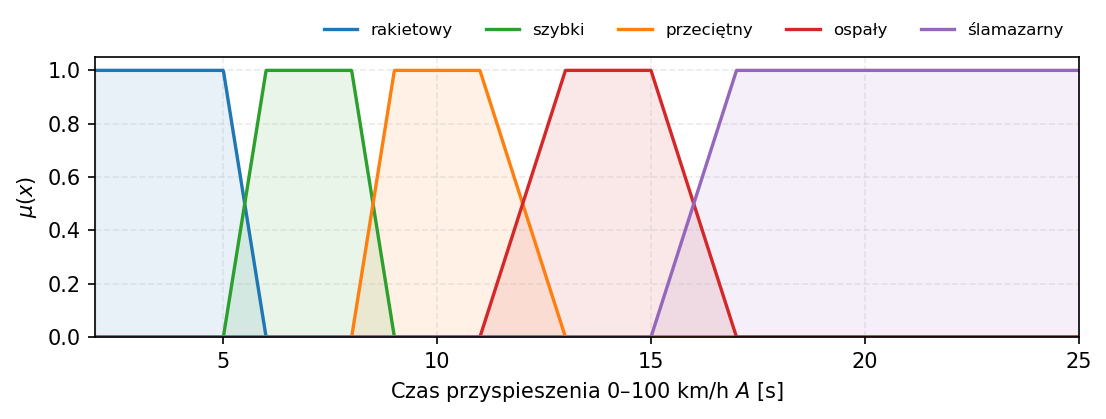
\includegraphics[width=0.9\textwidth]{mf_acceleration_0_100_s.png}
\caption{Funkcje przynależności pięciu etykiet zmiennej lingwistycznej
,,czas przyspieszenia 0--100~km/h'' $A \in [2, 25]$~s. Niskie wartości
$A$ ($<$5~s) odpowiadają samochodom szybkim, wysokie ($>$15~s) --
samochodom wolnym.}
\label{fig:mf-accel}
\end{figure}

\begin{figure}[H]
\centering
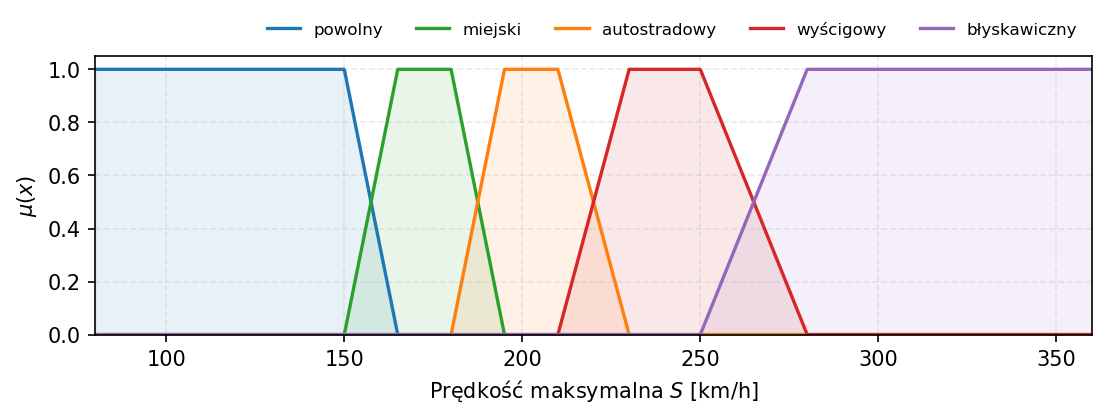
\includegraphics[width=0.9\textwidth]{mf_max_speed_km_per_h.png}
\caption{Funkcje przynależności pięciu etykiet zmiennej lingwistycznej
,,prędkość maksymalna'' $S \in [80, 360]$~km/h.}
\label{fig:mf-vmax}
\end{figure}

\begin{figure}[H]
\centering
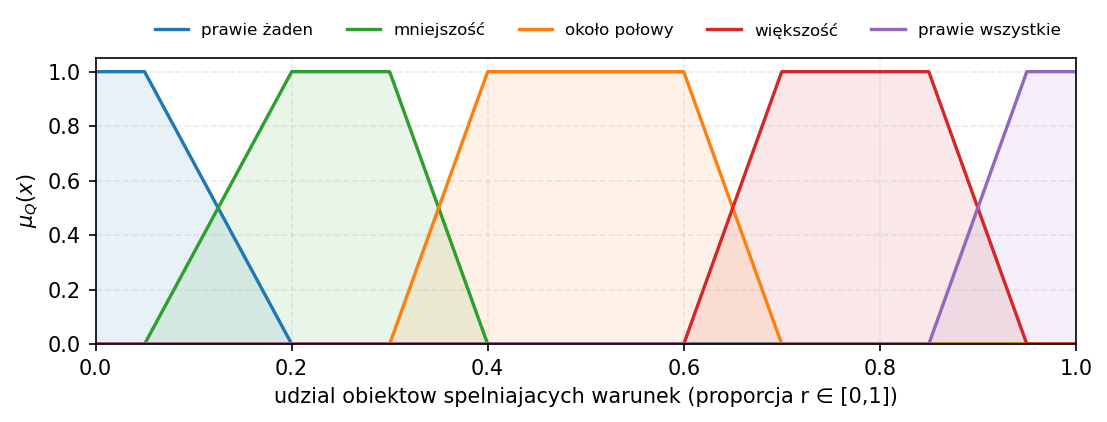
\includegraphics[width=0.9\textwidth]{quantifiers_relative.png}
\caption{Funkcje przynależności pięciu kwantyfikatorów względnych
zdefiniowanych na przestrzeni $X_Q = [0, 1]$. Argumentem
jest proporcja obiektów spełniających warunek (np. $r=0{,}5$:
$\mu_{\text{około połowy}}=1$).}
\label{fig:quant-rel}
\end{figure}

\begin{figure}[H]
\centering
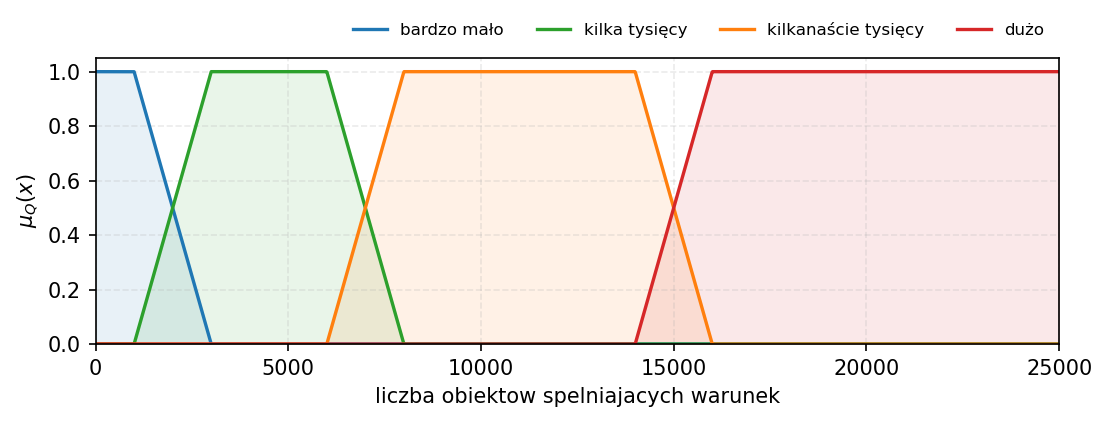
\includegraphics[width=0.9\textwidth]{quantifiers_absolute.png}
\caption{Funkcje przynależności czterech kwantyfikatorów bezwzględnych
zdefiniowanych na przestrzeni $X_Q^{\text{abs}} = [0, 25\,000]$.
Argumentem jest liczba obiektów spełniających warunek.}
\label{fig:quant-abs}
\end{figure}

\end{document}
